In questa ultima sezione ci occupiamo di progettare la parte del software che permetterà la visualizzazione del percorso (calcolato in precedenza), sulla mappa, con le eventuali fermate da effettuare.

\section{Progettazione dei Test} 
\hypertarget{section::\theHsection}
Sappiamo che la funzione che si occuperà di disegnare il tragitto dovrà prendere in input le coordinate dei punti di sosta, creare i marker sulla mappa, tracciare il percorso e restituire un valore booleano. Sappiamo inoltre che all'interno di questa funzione ci saranno diversi \textit{if statements}, quindi ci assicuriamo di testare le varie casistiche che si svilupperanno in fase di esecuzione.

\section{Pseudocodice} 
\hypertarget{section::\theHsection}
Di seguito è riportato in pseudocodice la parte di visualizzazione del percorso sulla mappa. \autocite[\protect\label{Zammetti2007}][]{Zammetti2007}
\lstinputlisting[language=JavaScript]{Codice/pseudocode_displayResults.pseudo}

\begin{figure}[htp]
\centering
{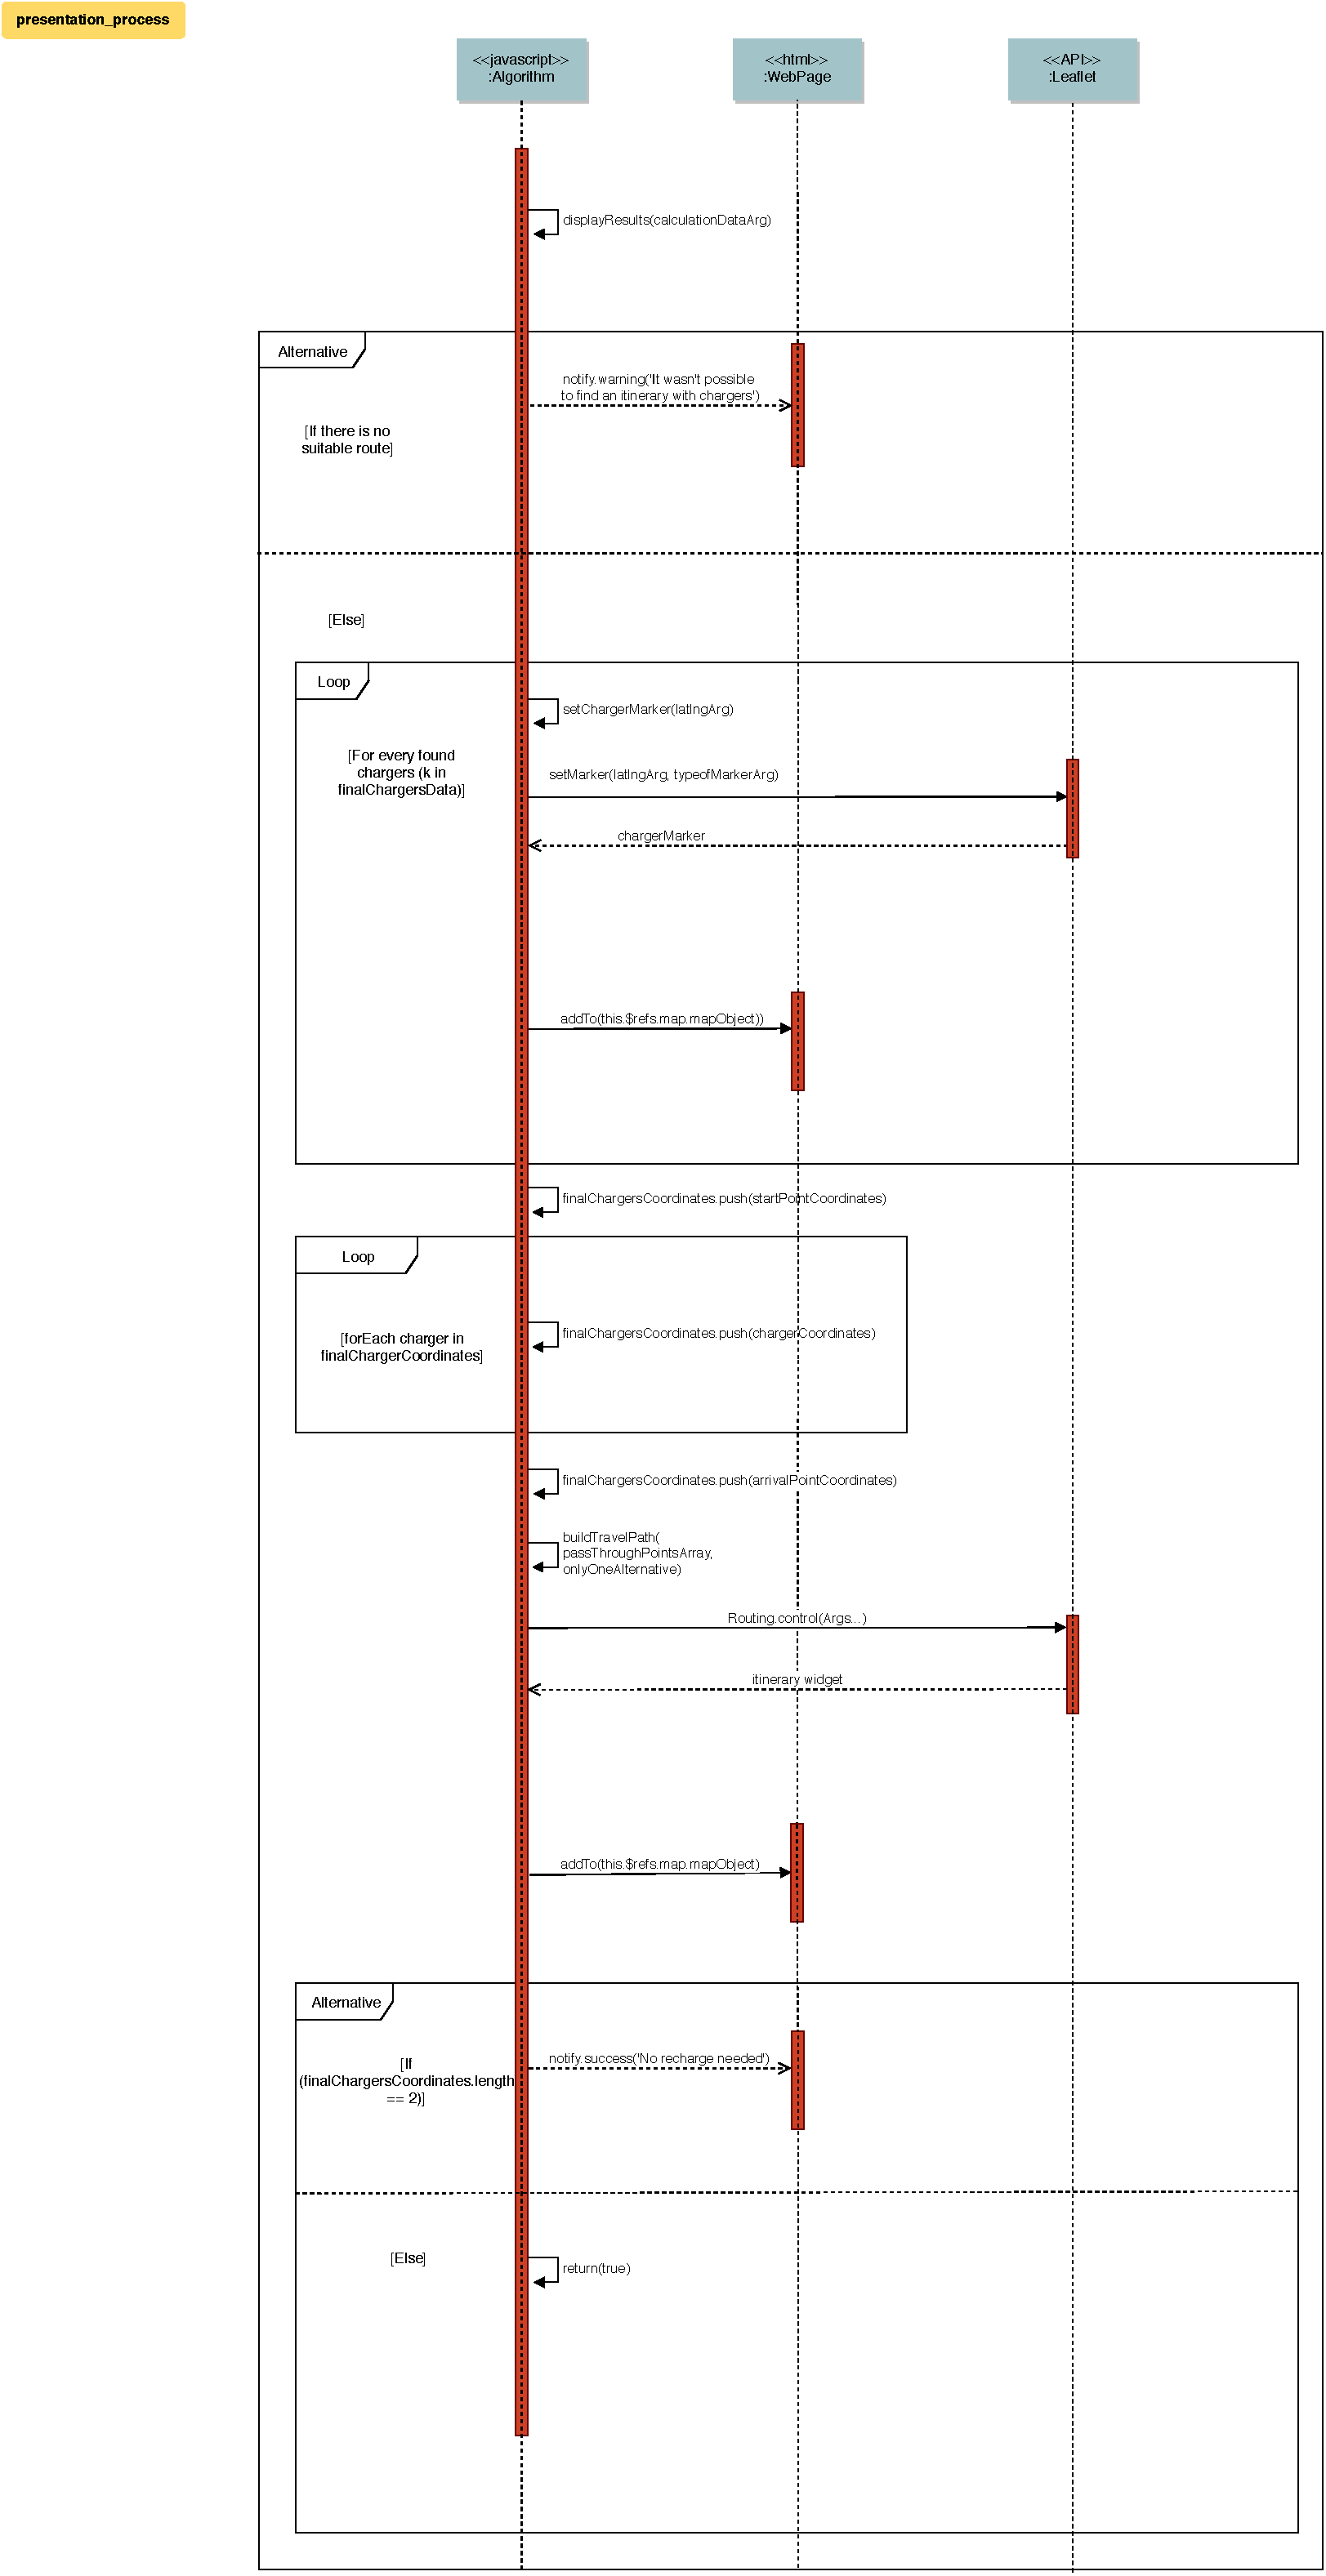
\includegraphics[scale=0.35]{Immagini/Presentation_SequenceDiagram.pdf}}
\caption{Template Deployment Diagram}
\end{figure}

\newpage

\section{Risultato dei Test} 
\hypertarget{section::\theHsection}
Il risultato dei test per questa iterazione è mostrato in figura. La suite composta da 3 test ha ricevuto esito positivo.

\begin{figure}[H]
\centering
{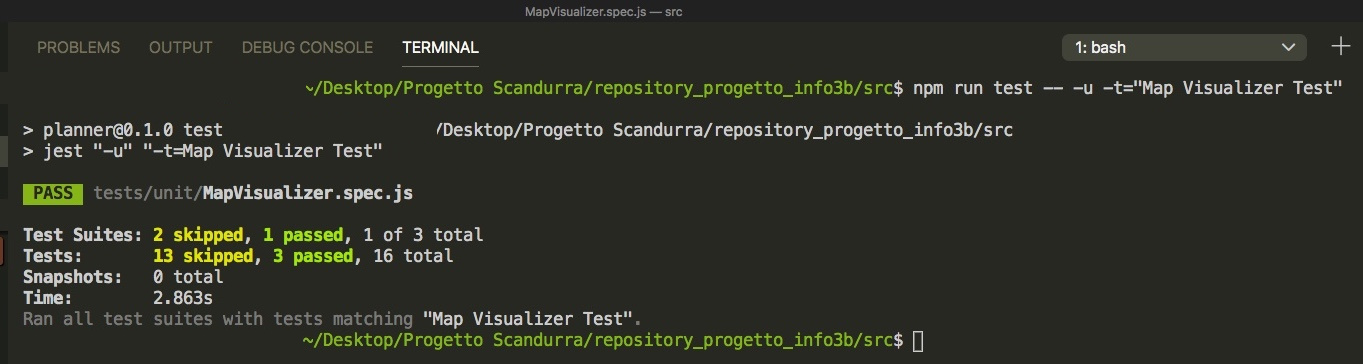
\includegraphics[scale=1]{Immagini/TestMapVisualizer.jpeg}}
\caption{Test iterazione 3}
\end{figure}

Presentiamo infine anche il risultato di tutte le suite di test per tutte le iterazioni eseguite contemporaneamente.

\begin{figure}[H]
\centering
{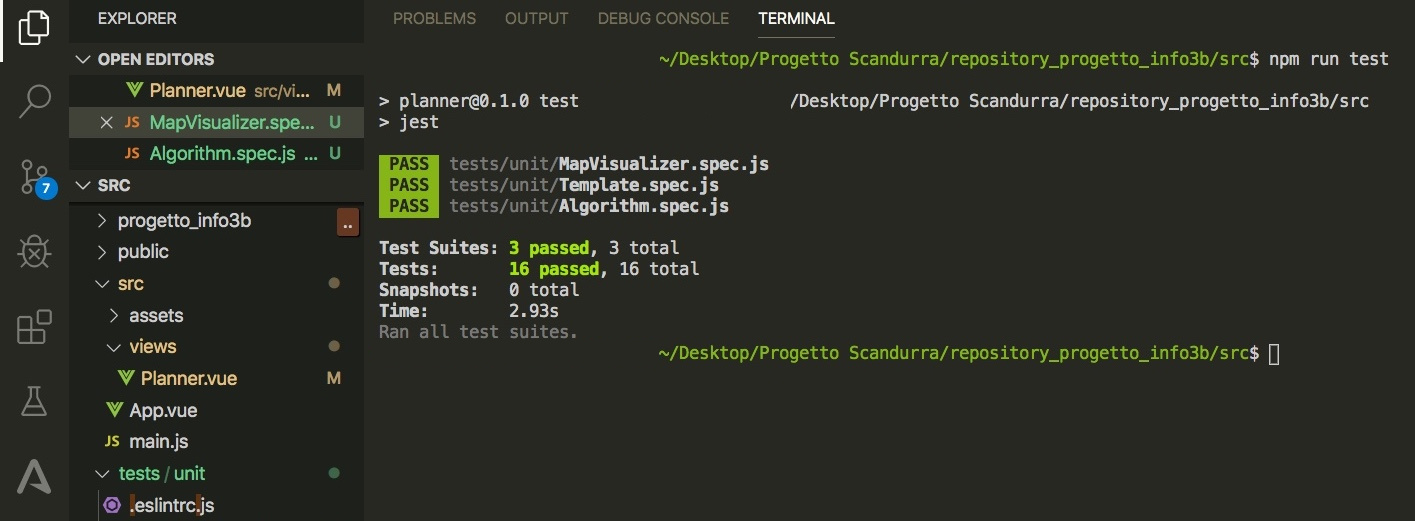
\includegraphics[scale=1]{Immagini/TestTotale.jpeg}}
\caption{Test completo}
\end{figure}
